\section{Introduction}
Long-lived particles (LLPs) are particles with lifetime comparable to particles at weak scale in Standard Model (SM). LLPs exist in Standard Model and commonly predicted in beyond Standard Model (BSM) physics. 

The long lifetime can arise from multiple reasons, including approximate symmetries that stabilize the LLPs, small coupling which narrow the decay widths of LLPs, and suppressed phase space for final state \cite{alimena2019searching}. In some cases, more than one reason can combine and lead to long lifetime in both SM and BSM. Since the proper decay lengths,$c\tau$, of LLP is comparable to the size of detector, the signatures are exotic in collider physics and distinguishable between SM and BSM. For the above properties, experimental signatures of LLPs in LHC are good probe for the search of new physics (NP) while are varied and complex. For example, LLPs signatures can include disappearing, appearing, and kinked tracks, displaced vertices and jets in inner detector, calorimeter, and muon system region, as well as trackless localized energy deposits in calorimeters. The behaviors of LLP signatures are summarized in Fig.\ref{fig:LLPsignature}

\begin{figure}[!h]
    \centering
    \caption{Schematic of the variety of challenging, atypical experimental signatures that can result from BSM LLPs in the detectors at the LHC. Shown is a cross-sectional plane in azimuthal angle, $\phi$, of a general purpose detector such as ATLAS or CMS. From \cite{russell2017llp}}
    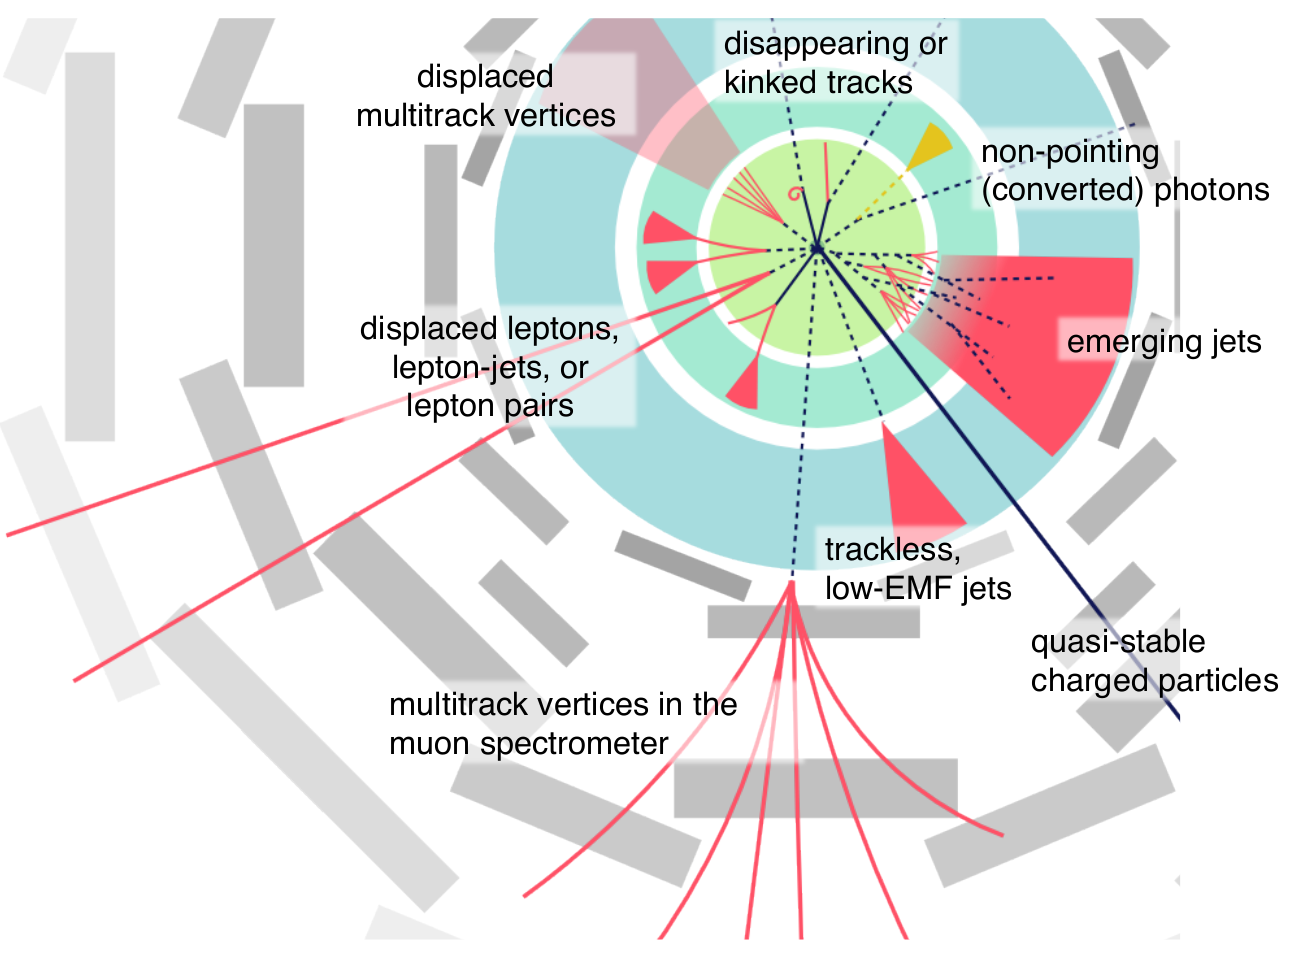
\includegraphics[width=0.5\textwidth]{fig/LLPSignature.png}
    \label{fig:LLPsignature}
\end{figure}

Although the LLP signatures are distinguishable from SM signatures, standard reconstruction algorithm developed for SM process may reject events with LLP signatures due to their unusual behaviors and dedicated analysis are necessary. These signatures also resemble background including detector noise, pile-up particles, and mis-reconstructed objects which is inaccurate in  Monte Carlo (MC) simulation. It is a challenge to model all sources of background and  make precise estimation in LLP searches. Furthermore, triggers and algorithms optimized for LLP signatures should be applied to simplify searches in future.

Heretofore, many searches for LLPs have been performed at the Large Hadron Collider (LHC). Detailed searches are described in Chapter IV. Existing LLP searches prove the necessity of methods for identifying signals of LLP and vetoing backgrounds. 